\section{Preliminary Evaluation}
\label{eval}

%In this section, we describe our empirical evaluation on the detection
%accuracy of {\model} in comparison with the state-of-the-art,
%SVM-based approach by Sun {\em et al.}~\cite{davidlo10}. All of
%experiments were carried out on on a computer with CPU AMD Phenom II
%X4 965 3.0 GHz, 8GB RAM, and Windows~10.

%We also re-implemented the machine learning approach described in
%their paper~\cite{davidlo10} using SVM in LIBSVM tool.

%\subsection{Data Sets and Feature Extraction}

%\begin{table}[t]
%\centering
%\caption{Statistics of All Bug Report Data}
%    \begin{tabular}{lcrrr}
%    \hline
%    Project &  Time period &  Report &  Duplicate &  Term \\
%    \hline
%    Eclipse  &  06/29/2008 - 06/28/2010 & 6,100 & 981 & 22,558 \\
%    OpenOffice & 04/12/2010 - 04/10/2011 & 7,000 & 338 & 22,051 \\
%    Firefox  &  01/26/2011 - 04/11/2011 & 20,000 & 936 & 42,515 \\
%    Apache  &  11/19/2006 - 03/30/2011 & 10,000 & 494   & 34,850 \\
%    FreeDesktop &  01/25/2010 - 04/13/2011 & 10,000 & 543   & 33,068 \\
%    NetBeans    & 06/17/2010 - 04/13/2011 & 10,000 & 993 & 27,417\\
%    \hline
%    \end{tabular}%
%\label{data}
%\end{table}

%\begin{table}[t]
%\addtolength{\tabcolsep}{-3pt}
%\centering
%\small
%\caption{Statistics of All Bug Report Data}
%    \begin{tabular}{lcccccc}
%    \hline
%    Project &  Time period &  Report &  Dup  & Train & Test \\
%    \hline
%    OpenOffice & 01/01/2008 - 12/21/2010 & 31,138 & 3,371 & 200 & 3,171  \\
%    Moz. FireFox &  01/01/2010 - 12/31/2010 & 75,653 & 6,925 & 200 & 6,725 \\
%    Eclipse  &  01/01/2008 - 12/31/2008 & 45,234 & 3,080 & 200 & 2,880  \\
%    \hline
%    Apache  &  11/19/2006 - 03/30/2011 & 10,000 & 494   & 200 & 3,485 \\
%    FreeDesktop &  01/25/2010 - 04/13/2011 & 10,000 & 543   & 200 & 3,306 \\
%    NetBeans    & 06/17/2010 - 04/13/2011 & 10,000 & 993 & 200 & 2,741\\
%    \hline
%    \end{tabular}
%\label{data}
%\end{table}



%We used the same data sets of bug reports in the open-source projects
%as in REP~\cite{sun-ase11} (Table~\ref{data}). 

%Column \code{Time period} displays the time period of collected bug
%reports. Columns \code{Report} and \code{Dup} show the numbers of bug
%reports and duplicate ones, respectively. Columns \code{Train} and
%\code{Test} show the number of the duplicate bug reports used for
%training and testing, respectively. Each bug report has its unique
%ID, a summary, a description, comments, and other metadata
%(e.g., severity, priority, its reporter, creation date, etc). All
%projects are developed in a long history.  
%The information on the duplications is available in the 
%collected bug reports. 
%Each duplicate report is marked and links to its duplicate group. The
%data is used to train {\model} and ensemble weights, and then used to
%evaluate {\model}'s accuracy in detecting the duplication between a
%bug report and the duplicate bug report~groups.
%-------------------------------------------------

%We conducted an empirical evaluation of {\model} on several
%open-source systems. We collected the data from the bug repositories
%of the systems (Table~\ref{data}). Column \code{Time period} displays
%the time period of collected bug reports. Columns \code{Report} and
%\code{Duplicate} show the numbers of bug reports and duplicate ones,
%respectively.
%For Eclipse, we chose Eclipse' s platform component from October 2000
%to July 2010 with 61,110 bug reports, in which 14,020 are determined
%by Eclipse's developers as duplicate ones. For Jazz project from June
%2005 to June 2008, the total number of bug reports are 34,228, in
%which 874 of them are recorded as duplications. 
%Each bug report has its unique ID, a summary, a description, comments,
%and other metadata (e.g. severity, priority, its reporter, creation
%date, platform, etc).

%The summary and description of a bug report were merged and considered
%as a document. It then went through pre-processing such as stemming,
%and removing grammatical and stopwords, and single-occurrence words
%as in~\cite{davidlo10}.
%In our experiment, for {\model}, we extracted and merged the summary
%and description of each report, and used the merged contents as the
%document for the report. Each document was then preprocessed such as
%stemming for term normalization, and removing grammatical words
%(e.g., ``a'', ``the'', ``and'', etc.) and those terms appearing once in
%the entire corpus as in~\cite{RTM}. Tf-Idf was run to determine and
%remove the common words that appear in most of the bug reports.
%Then, all the words were collected and indexed into a vocabulary.
%After this phase, a bug report is represented as a vector of the
%indexes of its words in the vocabulary. After this phase, a bug report is
%represented as a vector of indexes of its words in the vocabulary and
%is used in the model. Duplication information among bug reports was
%also extracted from the repositories.

%In our experiment, we extracted and merged the summary and description
%of each report, and used the merged contents as the document for the
%report. Each document was then preprocessed such as stemming for term
%normalization, and removing grammatical words (e.g. ``a'', ``the'',
%``and'', etc) and those terms appearing once in the entire corpus as
%in~\cite{RTM}.
%%%This phase include stemming for term normalization, removing
%%%grammatical words (e.g. ``a'', ``the'', ``and'', etc) and those that
%%%appear once in the entire corpus or appear in almost all
%%%documents.
%Then, all the words were collected and indexed into a vocabulary.
%Column \code{Term} shows the number of extracted terms in each
%vocabulary set after pre-processing. After this phase, a bug report is
%represented as a vector of indexes of its words in the vocabulary and
%is used in the model. Duplication information among bug reports was
%also extracted from the repositories.


%%%That is, a document of bug report $d$ with $N$ words will have the
%%%form ${\bf{w}}_d=(w_{d0}, w_{d1}, ..., w_{dN})$ where $w_{dk}$ is the
%%%index of the word at position $k$ in the vocabulary.
%%%The link indicator for $d$ with another bug report $d'$ will take the
%%%value of 1 if they are duplicate, otherwise, it will take the value of
%%%0. The vectors of bug reports and the values for the link indicators
%%%were used as features in training {\model}.

%This vector and the link indicator of the duplicate reports of $d$
%with all other known bug reports $d'$, which take value of $1$ if $d$
%is a duplicate of $d'$ and $0$ otherwise, will be applied to the input
%of iRTM.

\begin{figure}[t]
\centering
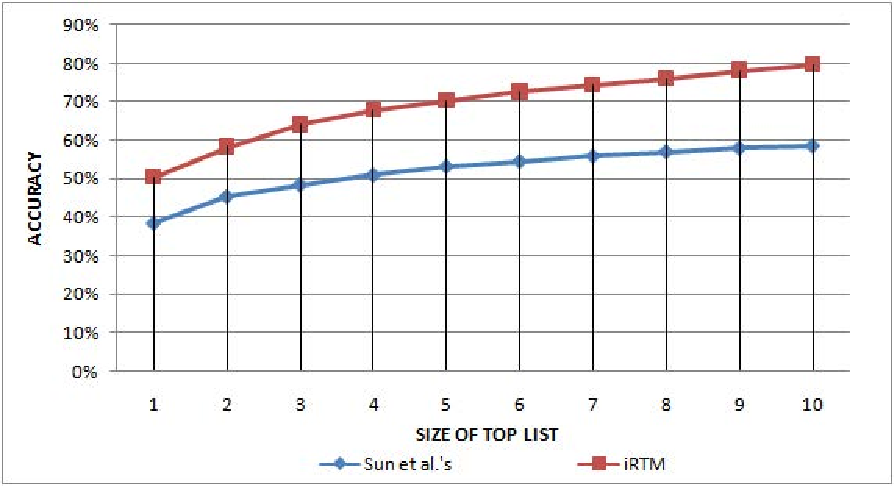
\includegraphics[width=3in]{eclipse3}
\caption{Accuracy Comparison with Different Top List Sizes}
\label{eclipse}
\end{figure}

We have conducted a preliminary evaluation on our model.
We chose the same data sets of bug reports used in
the existing work~\cite{davidlo10}. Due to the space limit, we will
not present the details of our experiment.
%In summary, our model can achieve up to 90\% top-10 accuracy, with
%updating time within 0.14 seconds per new bug report on average. The
%updating time for our model with new data is about 5-8 times smaller
%than the re-training time of the Sun {\em et al.}'s approach
%in~\cite{davidlo10}.
%Figure~\ref{eclipse} displays the accuracy result of our model in
%comparison with Sun {\em et al.}'s on Eclipse data set.
As seen in Figure~\ref{eclipse}, for a new bug report, {\bf in half of
  the detection cases, our model can correctly detect the duplication
  (if any) with just a single result}. With a list of top 5 resulting
bug reports, our model can correctly detect the duplication of a given
report in 71\% of the cases. That is, given a bug report, it can
correctly detect its duplication(s) (if any) within its top-5
recommended bug reports in almost 3 out of 4 cases. With top lists of
10 reports, it can correctly detect in 80\% of the cases. In
comparison, Sun {\em et al.}'s tool can achieve the accuracy levels at
the top lists of sizes 5 and 10 at only 53\% and 58\%,
respectively. In general, for top lists from 1-10 bug reports, {\bf
  our model achieves higher accuracy than Sun {\em et al.}'s from
  12--22\%}.



